\documentclass[11pt]{article}
\usepackage[utf8]{inputenc}
\usepackage[T1]{fontenc}
\usepackage{lmodern}
\usepackage{geometry}
\usepackage{microtype}
\usepackage{graphicx}
\usepackage{hyperref}
\usepackage{amsmath}
\usepackage{amssymb}
\usepackage{enumitem}
\usepackage{xcolor}

\geometry{margin=1in}
\hypersetup{
  colorlinks=true,
  linkcolor=blue!60!black,
  citecolor=blue!60!black,
  urlcolor=blue!60!black,
  pdfauthor={Lighthouse Research},
  pdftitle={Signals Protocol}
}

% Handy shortcuts
\newcommand{\signals}{\textsc{Signals}}
\newcommand{\todo}[1]{\textcolor{red}{[TODO: #1]}}


\title{Signals Protocol}
\author{Arnold Almeida \\ \texttt{arnold@lighthouse.cx} \and James MacWhyte \\ \texttt{james@lighthouse.cx}}
\date{\today}

\begin{document}
\maketitle

\begin{abstract}
Signals is a board-based on-chain coordination primitive where members lock an ERC-20 for time to express intensity of support on concrete initiatives. Each lock mints a transferable ERC-721 that represents the right to redeem the underlying after expiry or earlier upon initiative acceptance. Boards are immutable configurations at deployment time: lock interval, maximum lock duration (in intervals), decay curve and parameters, acceptance criteria (owner/anyone gating plus fixed and/or percentage thresholds), eligibility requirements for proposers and supporters, inactivity timeout, and optional post-acceptance release timelock. The protocol integrates optional reward mechanisms: a multi-board \texttt{IncentivesPool} that distributes board-wide participation rewards via time-bucketed weighting, and a per-initiative \texttt{Bounties} contract backed by an allow-listed \texttt{TokenRegistry}. Boards are deployed via a minimal-proxy factory and expose a simple lifecycle: propose, support (mint lock NFT), accept or expire, and redeem. This document preserves the system's motivation and design goals while grounding the mechanisms in the shipped contracts and validated behaviors from tests and docs.
\end{abstract}

\section{Introduction}
Signals is an on-chain protocol that converts latent community sentiment into a real-time, ranked idea board of DAO initiatives. Inspired by conviction voting\footnote{\cite{convictionvoting-cadcad, emmett2019conviction}.}, commitment voting\footnote{\cite{berg2020commitment, khezr2024bond}.}, and veToken systems such as Curve, Aragon, and Velodrome\footnote{\cite{curve-vecrv-understanding, curve-vecrv-overview, aragon2024mode, velodrome2022launch}.}, it lets members lock their existing governance tokens for a period of time to signal their support for what they think is most important. This token-time locking, coupled with configurable decay curves and acceptance thresholds, equips decentralized organizations with a transparent, mathematically grounded mechanism for continuous sensemaking.

We expect Signals to become an on-chain instrument for prioritizing structural changes and capital allocation while creating new utility for governance tokens.

\subsection{Goals}
\begin{itemize}[leftmargin=*]
  \item Deliver correctness and liveness guarantees under realistic network partitions.
  \item Keep the trust surface minimal and explicit.
  \item Make operational costs predictable for deployments of varying scale.
\end{itemize}

\subsection{Non-goals}
List out-of-scope items to avoid scope creep and clarify assumptions.

\section{Motivation}
Token-based voting captures binary preferences on formal proposals but does little to surface intensity. After a decade of on-chain experimentation, DAOs still struggle to translate intent into timely, accountable action. Common pain points include:
\begin{itemize}[leftmargin=*]
  \item Endless discussion threads with unclear next steps.
  \item Committees that drift or concentrate power.
  \item Fragmented knowledge bases that deter newcomers.
  \item Social pressure that favors incumbents over fresh ideas.
\end{itemize}

By leveraging preference intensity through time-lock commitments, \signals{} constructs a dynamic idea board where the most strongly supported initiatives rise naturally, keeping attention on what matters and when. Concretely, each position requires locking real tokens for time; supporters own an ERC-721 claim on those tokens and must wait for expiry (or success) to redeem, making opportunity cost explicit.

To counteract last-minute pile-ons and apathetic equilibria, the protocol optionally distributes participation rewards. A shared \texttt{IncentivesPool} funds supporters of accepted initiatives based on when they committed support (earlier commitments earn higher weight via time buckets), while a \texttt{Bounties} module lets contributors escrow targeted rewards per initiative. Both mechanisms aim to reward early, accurate signaling and raise the cost of low-conviction behavior without distorting the core lock-and-decay semantics.

\section{Related Systems}

\paragraph{Conviction Voting}
Holders stake without fixed locks; conviction builds the longer tokens stay committed and can be re-allocated at any time (which resets build-up). Proposals auto-execute once time-weighted conviction crosses an adaptive threshold tied to requested resources. It channels persistent conviction into binding, resource-allocating decisions.

\paragraph{Commitment Voting}
Voters lock tokens for a period to determine voting power. If their choice wins, tokens remain locked as committed; losing side unlocks immediately. Victory carries opportunity cost, so intensity matters. See \cite{berg2020commitment, khezr2024bond}.

\paragraph{veToken Systems}
veCRV, Aragon OSx gauges, and Velodrome require duration-based locks to earn voting power. Lock length boosts influence across all votes but does not capture intensity on a specific initiative. See \cite{curve-vecrv-understanding, curve-vecrv-overview, velodrome2022launch, aragon2024mode}.

\paragraph{Signals}
Signals borrows the idea of time-weighted commitment but applies it to a continuous idea board rather than a binary election. Unlike conviction voting, support decays deterministically at a board-defined interval and is bounded by a maximum lock duration. Unlike veToken systems, voting weight is scoped to a specific initiative via an ERC-721 lock position. Acceptance combines programmable thresholds with access control, and optional rewards are delivered by externalized modules to keep the core trust surface small.

\section{Mechanism Design}

\subsection{Initiatives, not Proposals}
\signals{} works with \emph{Initiatives}---ideas or actions seeking support. Initiatives live inside Boards (configuration sets), and DAOs can run multiple Boards with different parameters. Board configs are on-chain, so DAOs can govern them directly.

\subsection{Token-Locking}
Participants lock existing tokens for a chosen duration to express commitment; locking against an Initiative is not supported. Each lockup mints a transferable NFT bond redeemable when the lock expires, enabling secondary markets or other reputation measures. Boards typically use governance tokens but can target any ERC-20.

\subsection{Calculating Support}
Time is measured in Epochs (Board-defined). Longer locks provide more weight:
\begin{equation}
  S = T \times D^{k}
\end{equation}
where $S$ is support, $T$ is tokens locked, $D$ is duration in Epochs, and $k$ is an exponential bonus favoring longer commitments. Tuning $k$ prevents short, large locks from dominating and lets smaller holders compete by committing longer.

\begin{figure}[h]
  \centering
  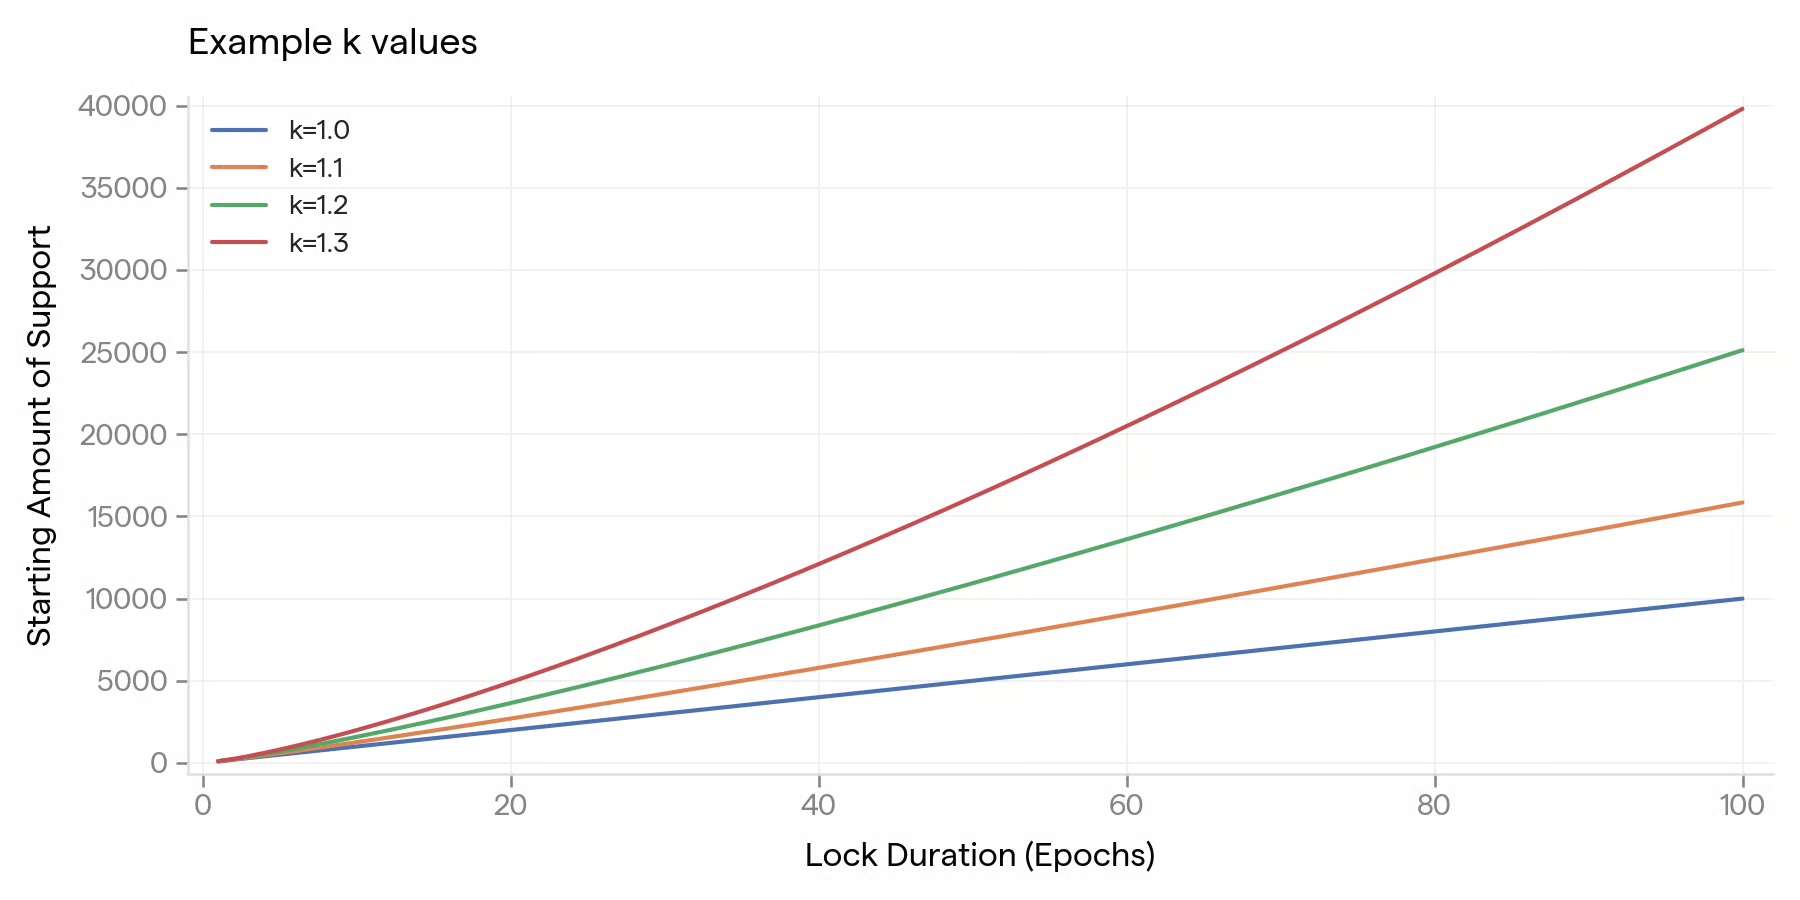
\includegraphics[width=0.85\linewidth]{figures/fig-boost-lockup.png}
  \caption{Adjusting $k$ changes how much additional weight longer lockups receive.}
\end{figure}

\subsection{Decay}
Support decays over time to keep rankings current. Each Board specifies a decay curve (linear, exponential, or custom). Current support for Initiative $i$ at time $t$ sums decayed contributions from its locks $\ell$:
\begin{equation}
  \text{CurrentSupport}_i(t) = \sum_{\ell \in \text{Locks}_i} \text{Weight}(\ell, t).
\end{equation}
Decay ensures abandoned initiatives fade, early interest provides a head start (not permanence), and manipulation via stale locks is limited.

\subsection{Actioning Initiatives}
Boards define an acceptance threshold. When current support exceeds it, an Initiative can be actioned: the Initiative closes and all supporting tokens unlock early. DAOs decide whether actioning is automatic or requires a trigger (committee, vote, or other mechanism). The early unlock incentivizes backing only initiatives expected to succeed.

\subsection{Examples of Support and Thresholds}
\begin{figure}[h]
  \centering
  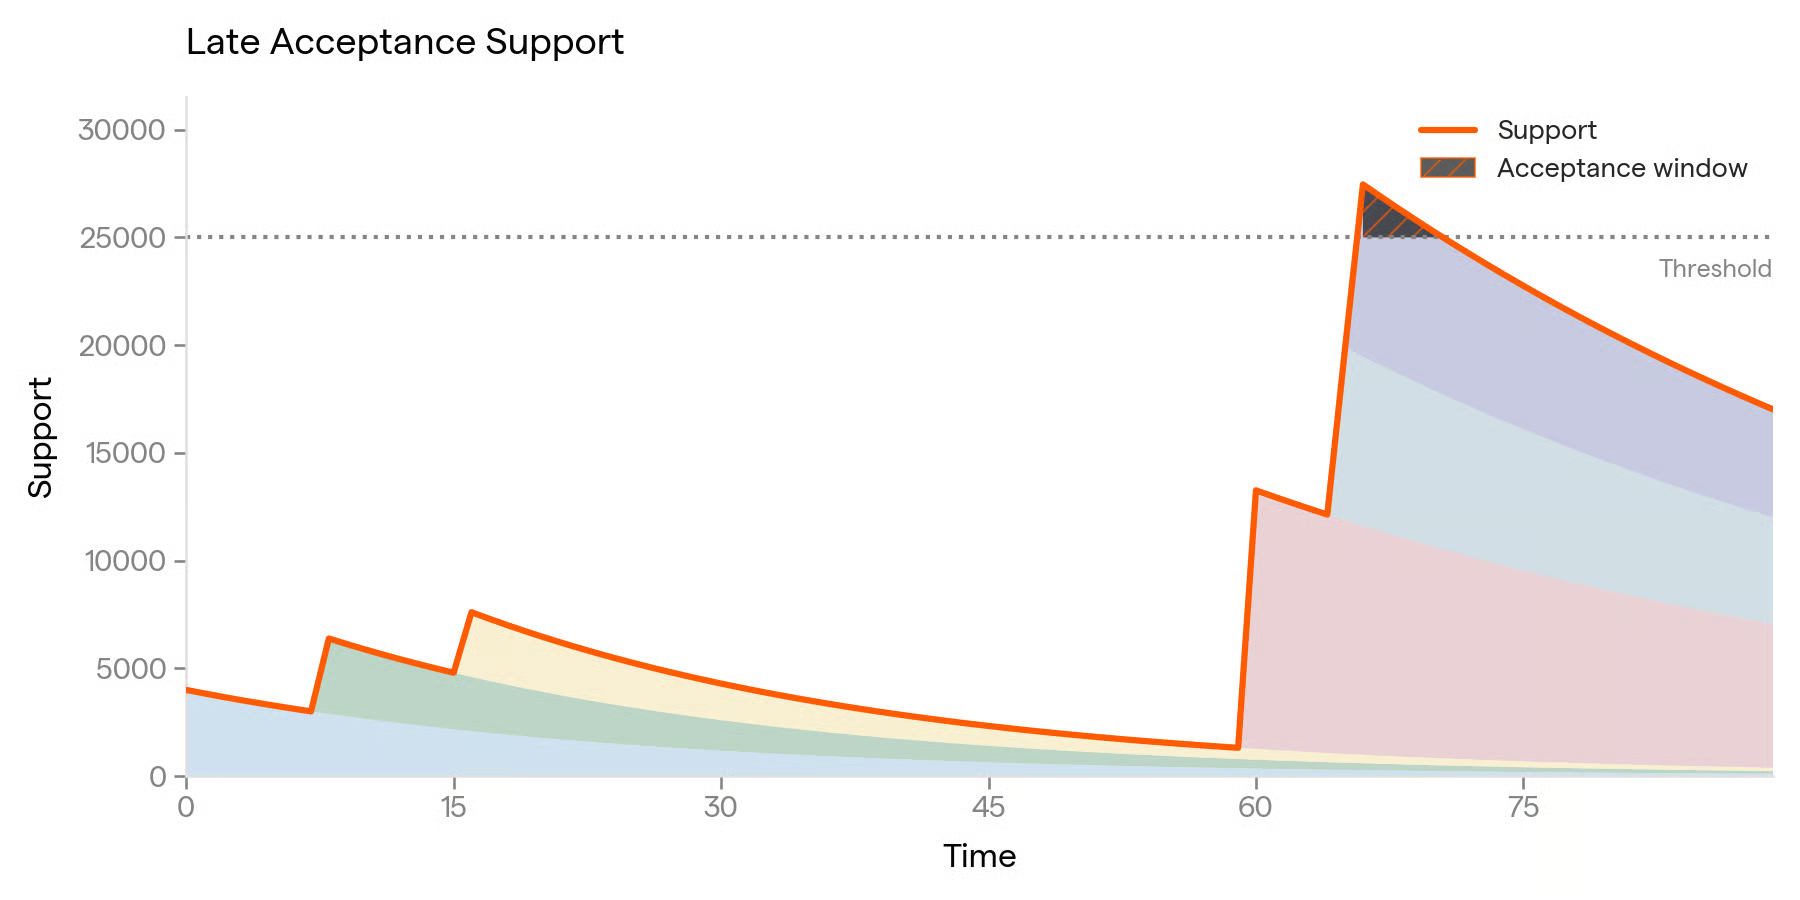
\includegraphics[width=0.85\linewidth]{figures/fig-late-acceptance.png}
  \caption{Early support is insufficient; renewed interest later can re-open the path to action.}
\end{figure}

\begin{figure}[h]
  \centering
  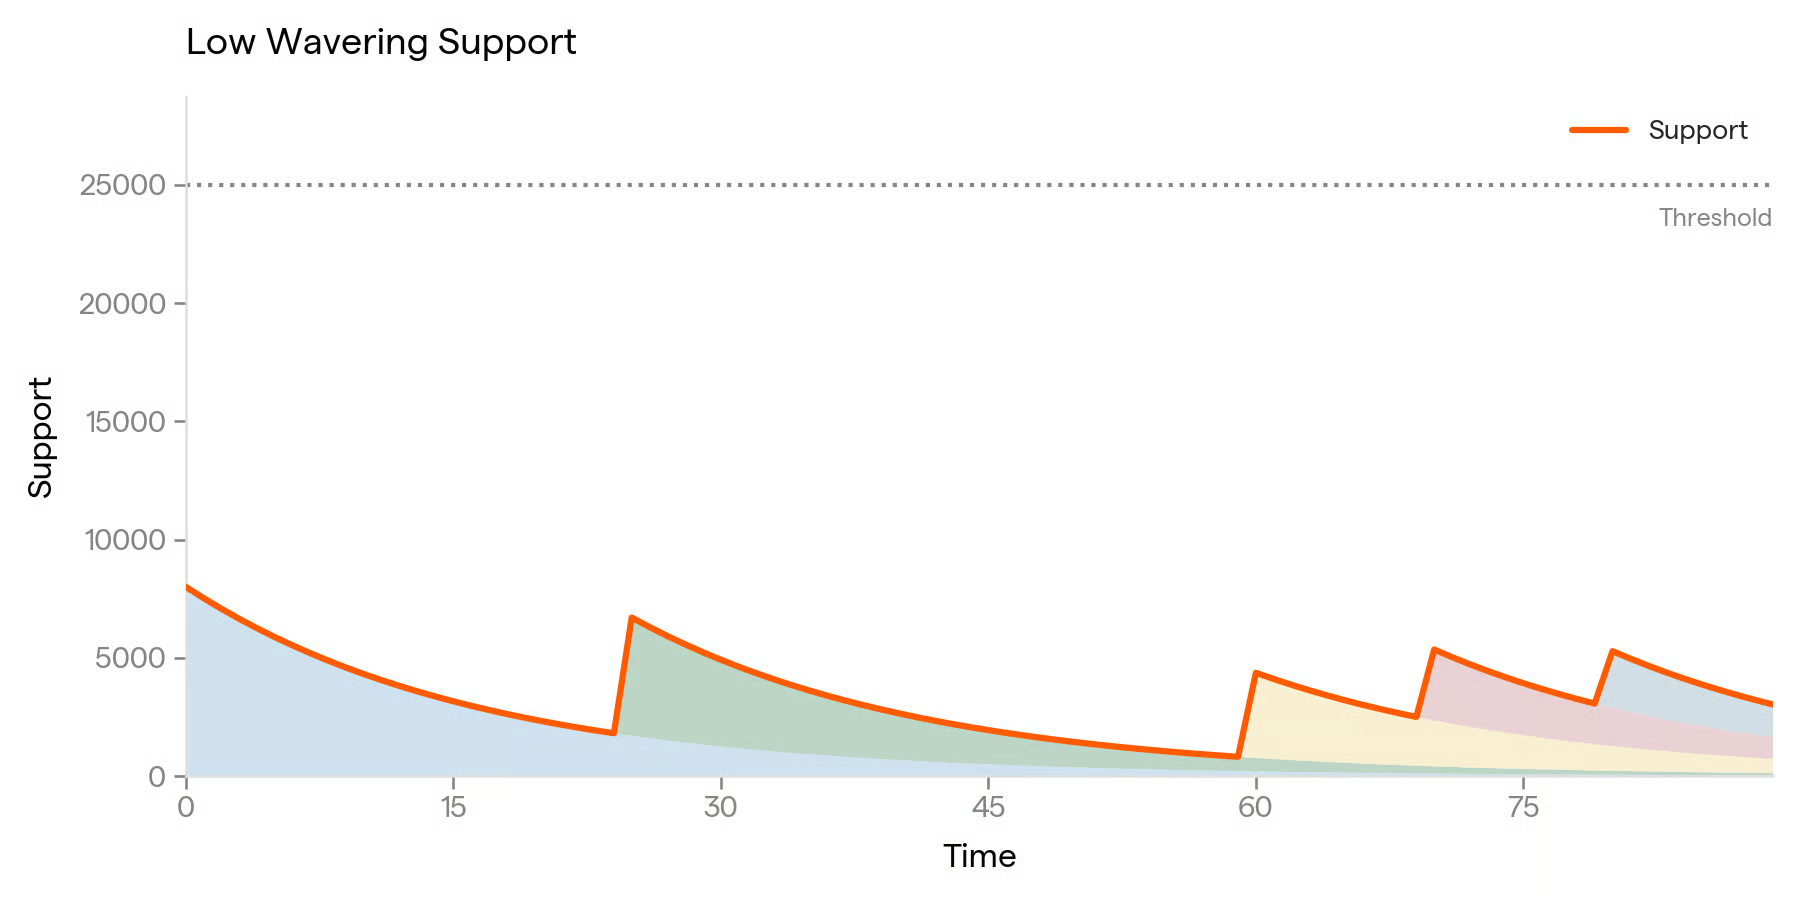
\includegraphics[width=0.85\linewidth]{figures/fig-low-wavering-support.png}
  \caption{Insufficient, wavering support never crosses the threshold despite cumulative effort.}
\end{figure}

\begin{figure}[h]
  \centering
  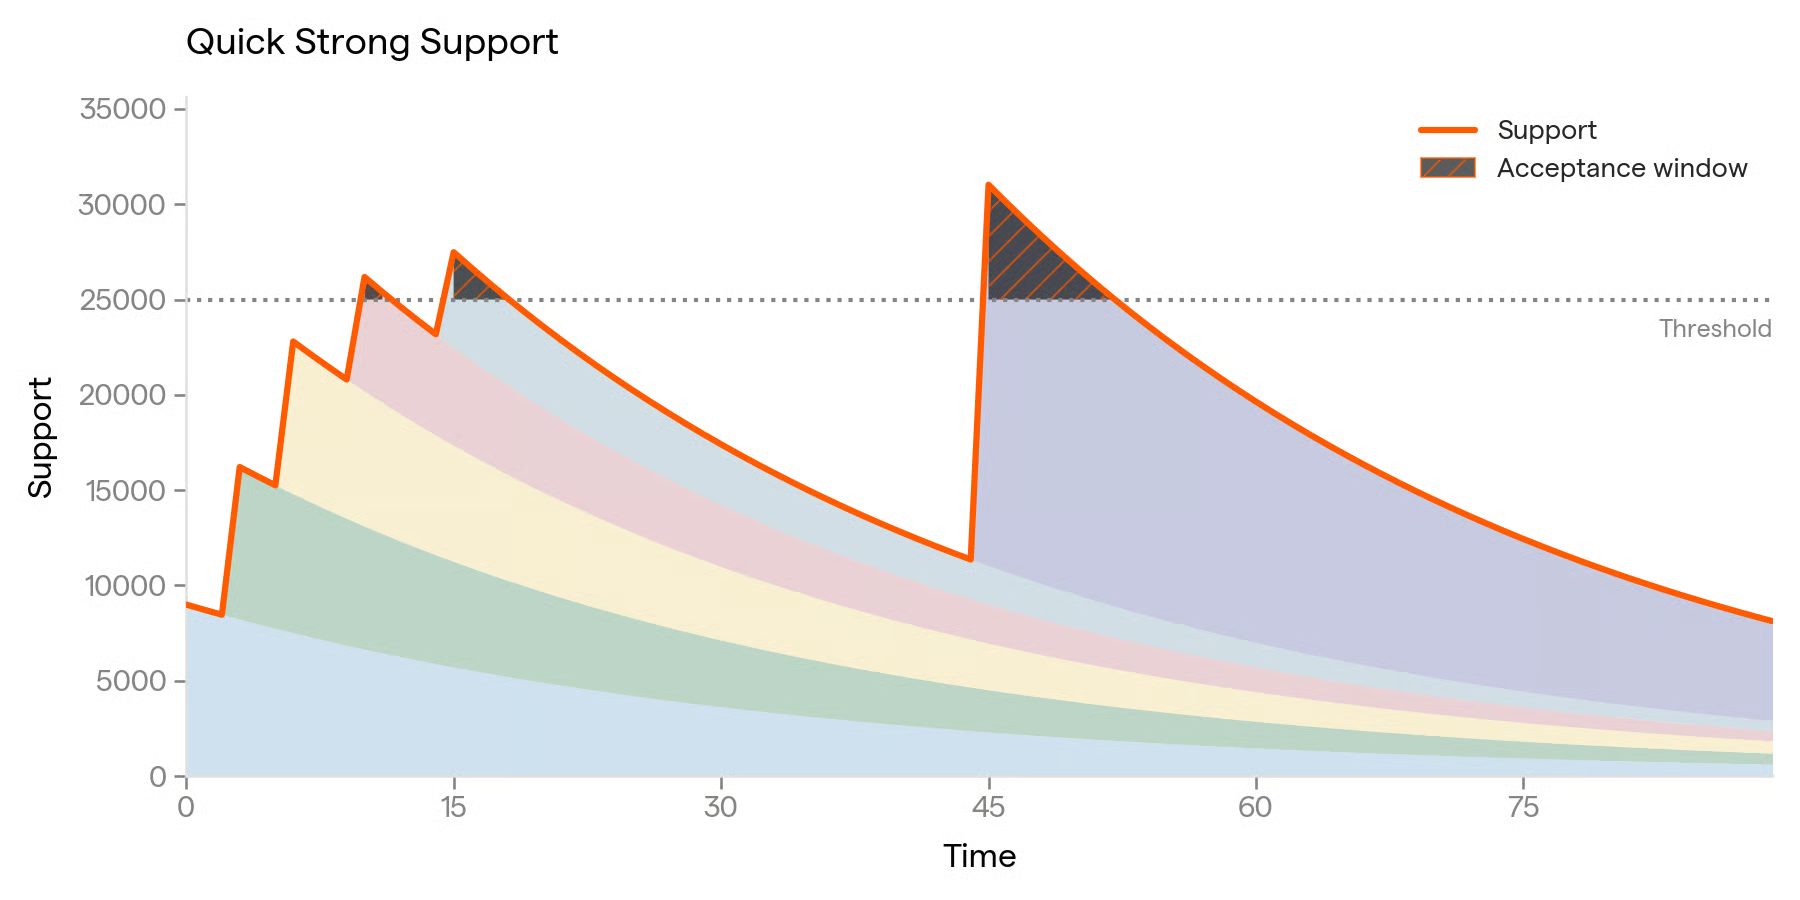
\includegraphics[width=0.85\linewidth]{figures/fig-quick-support.png}
  \caption{Late momentum pushes an Initiative over the threshold after an initial lull.}
\end{figure}

\subsection{Endorsements (Optional)}
If a DAO uses delegated voting, delegates may not own the tokens they wield. Boards can optionally require binary \emph{Endorsements} tied to delegated voting power in addition to lockups. Caps on endorsements per Initiative encourage delegates to act early and visibly.

\section{Paid Incentives in Signals}
\subsection{Motivation}
DAOs often face low participation: most holders do not see sufficient upside to engage, and reputational risk pushes signaling to the last minute. Some DAOs spend \$1M+ per year on delegate programs. Signals inherits similar participation risks, so we add configurable incentives that reward early, accurate support and penalize weak or misaligned signaling.

\subsection{Mechanism 1: General Participation Incentives (IncentivesPool)}
A shared \texttt{IncentivesPool} can fund supporters of any initiative that gets accepted. The pool is independent from boards and can be shared across many (1:M). Its reward token is immutable and specified in the constructor; funds are added with \texttt{addFundsToPool}. Boards must be explicitly approved with two parameters: a per-board \emph{max budget} and a \emph{totalRewardPerInitiative} cap. Boards then link to the pool \emph{before} they open.

When supporters add locks, the board records each lock's \emph{incentive credit} in the pool using the lock's time-weighted contribution at creation. Credits are aggregated into a fixed number of time buckets (default: 24) with a starting interval (default: 1 hour). The board provides an \emph{incentive curve} configuration (linear today, 2--24 parameters), and the pool converts the curve into per-bucket multipliers via interpolation and normalization. On redemption after acceptance, the board requests the pool to pay rewards for the redeeming locks: each lock gets a share proportional to its credited bucket and the curve's multipliers. The pool enforces the per-initiative cap and the board's remaining budget; if depleted, payouts simply become zero without blocking acceptance or redemption.

\begin{itemize}[leftmargin=*]
  \item \textbf{Setup}: deploy pool with \texttt{REWARD\_TOKEN}, fund with \texttt{addFundsToPool}, approve boards with \texttt{approveBoard(board, boardBudget, totalRewardPerInitiative)}, link from the board before opening via \texttt{setIncentivesPool}.
  \item \textbf{Accounting}: time is bucketed and compressed (if buckets fill, they are reduced in-place to keep a bounded history).
  \item \textbf{Safety}: only approved boards can record credits and claim. Claims respect budgets and never revert for insufficient pool balance; rewards may be 0 if exhausted.
\end{itemize}

\subsection{Mechanism 2: Sponsored Initiative Incentives (Bounties)}
Anyone can add rewards to a specific initiative via the \texttt{Bounties} contract. Tokens must be on a \texttt{TokenRegistry} maintained by role-based access control. Bounties are stored with amount, optional expiration, and distribution \emph{splits} configured by the owner (e.g., protocol/treasury/supporters). On acceptance, bounties are aggregated by token and split according to the active version of the configuration, crediting internal balances for recipients. Current limitations: refunding expired bounties is a planned enhancement and is not fully implemented yet.

\subsection{Impact}
Rewards amplify Signals’ core design: only positive support, opportunity cost via locks, and time-weighted influence that lets smaller holders compete. Incentives raise the cost of frivolous signaling and make early, accurate support economically meaningful, improving resilience against brigading or apathy-driven noise.

\begin{figure}[h]
  \centering
  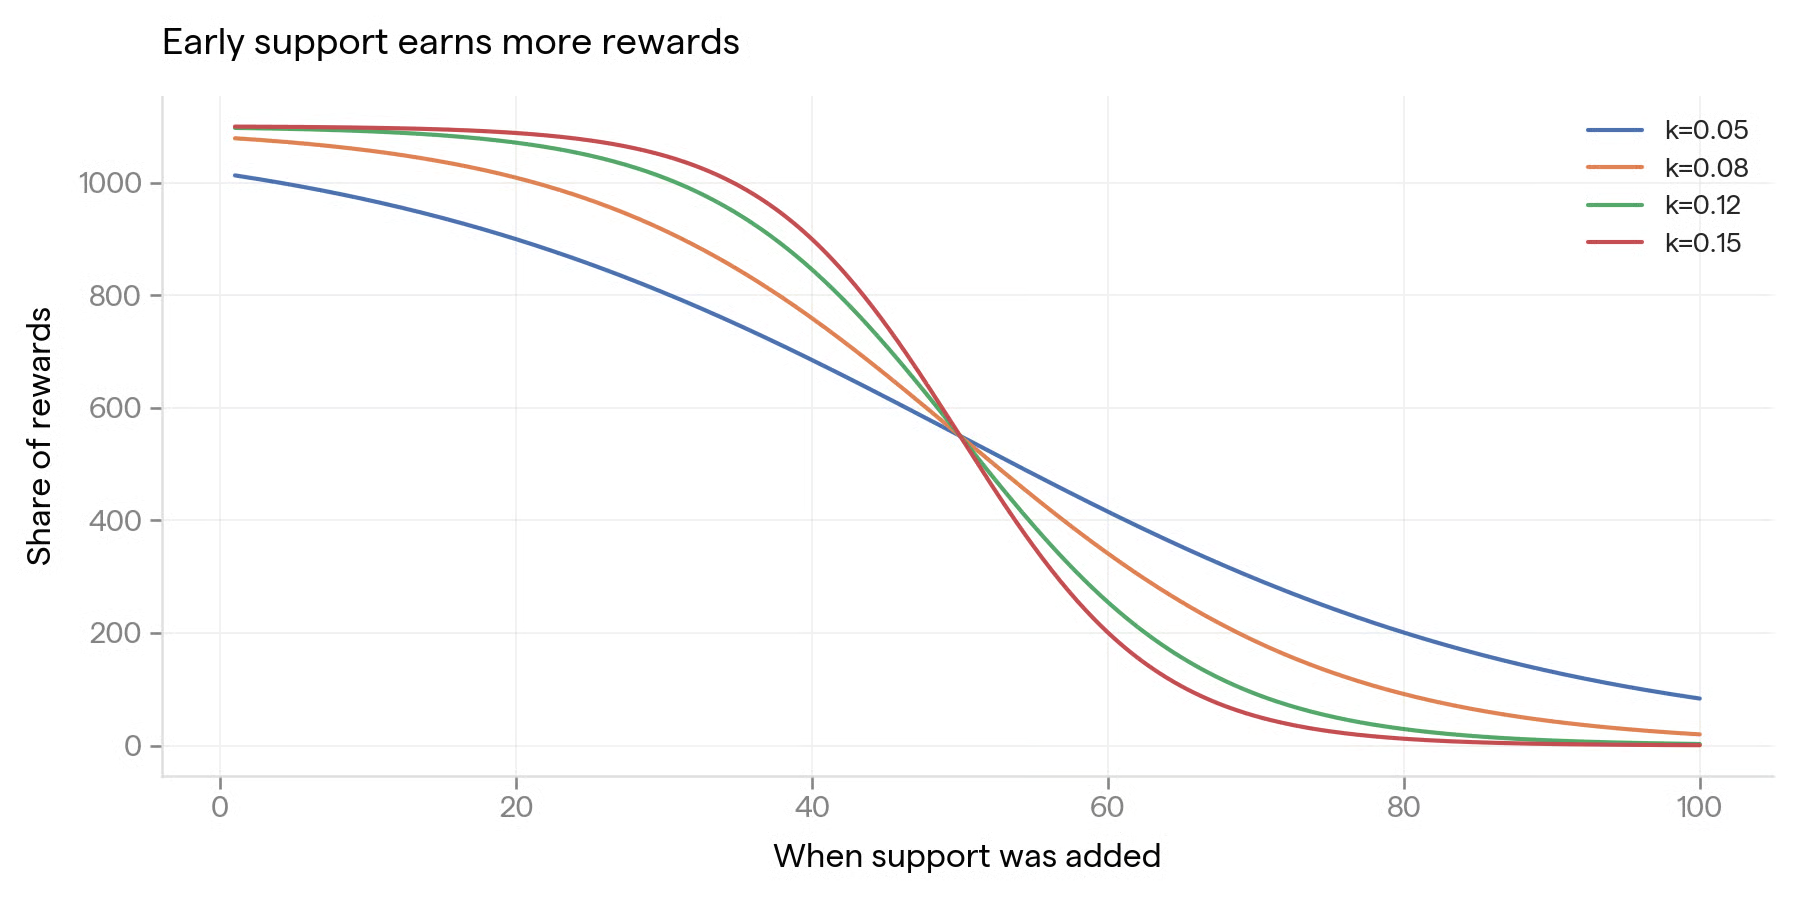
\includegraphics[width=0.85\linewidth]{figures/fig-rewards.png}
  \caption{Example reward distribution emphasizing early supporters via bucket multipliers and shared upside.}
\end{figure}

\subsection{Implementation Notes (from Tests)}
End-to-end tests validate:
\begin{itemize}[leftmargin=*]
  \item Linking a board to a pool must happen before the board opens; otherwise calls revert.
  \item Reward distribution with a single supporter pays the \texttt{totalRewardPerInitiative} cap (subject to remaining budget).
  \item With multiple supporters at different times, earlier buckets receive higher multipliers (per linear config) and split rewards accordingly.
  \item Pool depletion is non-blocking: acceptance and redemption succeed; claims pay zero if budgets are exhausted.
\end{itemize}

\section{What's Next}
The Signals proof of concept was built during the Arbitrum Collabtech Hackathon (1st place) and continued in the Uniswap Hooks Incubator (prizes from Arbitrum and the Uniswap Foundation). Contracts and dashboard are open source.\footnote{\url{https://github.com/0xLighthouse/signals}}

We aim to formalize and validate the protocol on:
\begin{itemize}[leftmargin=*]
  \item Capturing voter preference intensity and opportunity cost as sufficient risk.
  \item Locking as sybil resistance and its limits.
  \item Gameable vs. productive patterns for endorsements and reputation.
  \item Inclusivity: how smaller voting blocks benefit from time-weighted designs.
\end{itemize}

If interested in collaborating on a whitepaper, please reach out.


\bibliographystyle{plain}
\bibliography{references}
\end{document}
